% !TeX root = ./0Base.tex

\chapter{Results}\label{cha:results}

\section{Performance}

Graphs below (figures \ref{tab:resultsGet}, \ref{tab:resultsGetMany}, \ref{tab:resultsDelete}, \ref{tab:resultsPost} and \ref{tab:resultsPut}) show an average response time in milliseconds by number of concurrent \acrshort{vu}s from the tests mentioned in previous chapters. To better show the results of the tests, on vertical axis a logarithmic scale has been used, as Django had very long response times in comparison to other two frameworks. Under each graph there is a table with data used to draw the mentioned graphs - average response times rounded to second decimal place. As seen on the results, in cases with small amount concurrent requests Express.js application was the fastest. Starting from 32 \acrlong{vu}s for get requests, 128 for post and put requests and 512 for getMany ASP.NET Core has faster results. The trend line in all charts (except for delete tests, where ASP.NET is slower than express in all tests by from 8\% to 49\% depending on concurrency) shows that Express.js handles bigger loads worse than ASP.NET. In most tests Django stands out very far from the others, being even up to almost 17 times slower (for get tests with 8 concurrency) than the opponents. This framework surprised on getMany tests, where it was slower by only 15\% than the second best result - ASP.NET.

\begin{figure}[H]
    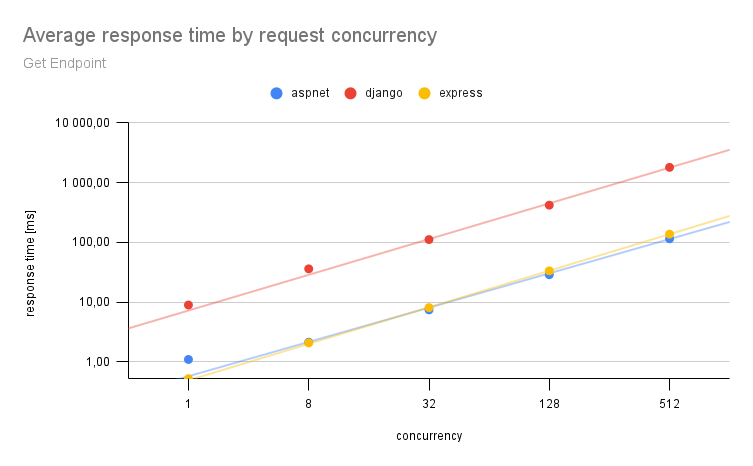
\includegraphics[width=\columnwidth]{figures/pictures/resultsGet.png}
    \caption{Average response time in get tests}
    \label{fig:resultsGet}
\end{figure}

\FloatBarrier
\begin{table}[!htp]\centering
    \caption{Average p(95) response time in tests}\label{tab:resultsGet}
    \scriptsize
    \begin{tabular}{lrrrrr}\toprule
        test & concurrency & aspnet & django   & express \\\midrule
        get  & 1           & 1.09   & 8.90     & 0.51    \\
        get  & 8           & 1.97   & 32.06    & 1.73    \\
        get  & 32          & 6.26   & 94.71    & 6.52    \\
        get  & 128         & 23.38  & 338.88   & 26.14   \\
        get  & 512         & 92.81  & 1,411.91 & 108.42  \\
        \bottomrule
    \end{tabular}
\end{table}
\FloatBarrier


\begin{figure}[H]
    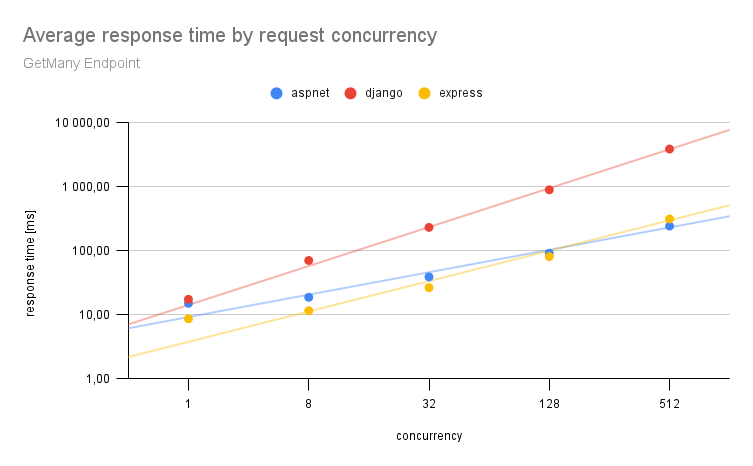
\includegraphics[width=\columnwidth]{figures/pictures/resultsGetMany.png}
    \caption{Average response time in getMany tests}
    \label{fig:resultsGetMany}
\end{figure}

\FloatBarrier
\begin{table}[!htp]\centering
    \caption{Average p(95) response time in tests}\label{tab:resultsGetMany}
    \scriptsize
    \begin{tabular}{lrrrrr}\toprule
        test    & concurrency & aspnet & django    & express \\\midrule
        getMany & 1           & 47.75  & 54.77     & 10.37   \\
        getMany & 8           & 42.03  & 267.56    & 11.72   \\
        getMany & 32          & 62.94  & 979.83    & 25.03   \\
        getMany & 128         & 112.69 & 3,897.61  & 69.38   \\
        getMany & 512         & 273.04 & 15,952.84 & 252.17  \\
        \bottomrule
    \end{tabular}
\end{table}
\FloatBarrier


\begin{figure}[H]
    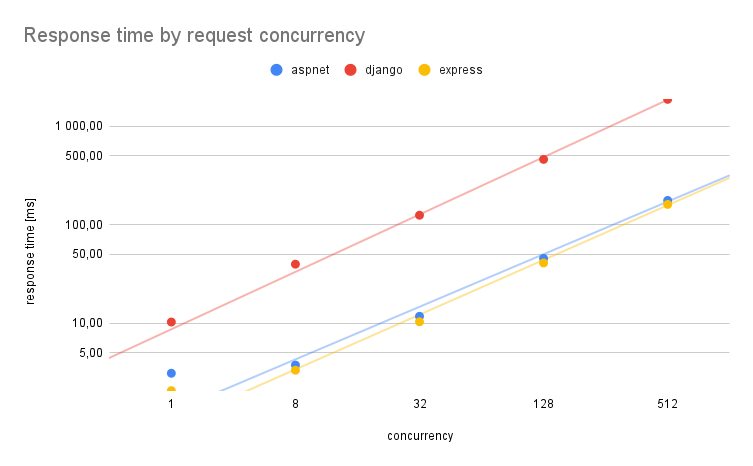
\includegraphics[width=\columnwidth]{figures/pictures/resultsDelete.png}
    \caption{Numeric results from delete tests}
    \label{fig:resultsDelete}
\end{figure}

\FloatBarrier
\begin{table}[!htp]\centering
    \caption{Average p(95) response time in tests}\label{tab:resultsDelete}
    \scriptsize
    \begin{tabular}{lrrrrr}\toprule
        test   & concurrency & aspnet & django   & express \\\midrule
        delete & 1           & 3.11   & 10.30    & 2.07    \\
        delete & 8           & 3.76   & 39.81    & 3.34    \\
        delete & 32          & 11.77  & 125.11   & 10.36   \\
        delete & 128         & 45.53  & 461.95   & 40.98   \\
        delete & 512         & 176.82 & 1,879.71 & 161.20  \\
        \bottomrule
    \end{tabular}
\end{table}
\FloatBarrier


\begin{figure}[H]
    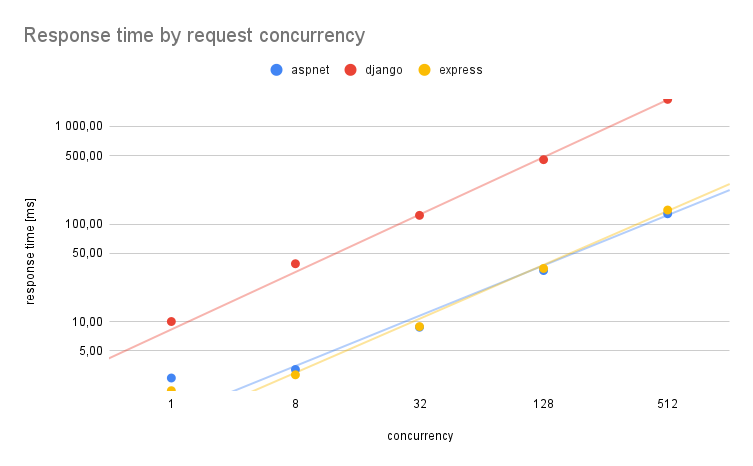
\includegraphics[width=\columnwidth]{figures/pictures/resultsPost.png}
    \caption{Numeric results from post tests}
    \label{fig:resultsPost}
\end{figure}

\FloatBarrier
\begin{table}[!htp]\centering
    \caption{Numeric results from post tests}\label{tab:resultsPost}
    \scriptsize
    \begin{tabular}{lrrrrr}\toprule
        test & concurrency & aspnet & django   & express \\\midrule
        post & 1           & 2.64   & 10.06    & 1.96    \\
        post & 8           & 3.29   & 45.23    & 3.02    \\
        post & 32          & 12.44  & 146.03   & 10.10   \\
        post & 128         & 38.54  & 564.70   & 40.40   \\
        post & 512         & 150.11 & 2,360.03 & 165.16  \\
        \bottomrule
    \end{tabular}
\end{table}
\FloatBarrier


\begin{figure}[H]
    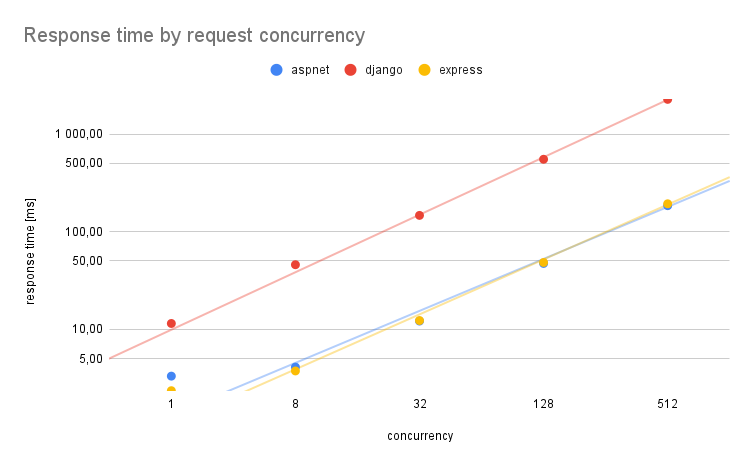
\includegraphics[width=\columnwidth]{figures/pictures/resultsPut.png}
    \caption{Numeric results from put tests}
    \label{fig:resultsPut}
\end{figure}

\FloatBarrier
\begin{table}[!htp]\centering
    \caption{Average p(95) response time in tests}\label{tab:resultsPut}
    \scriptsize
    \begin{tabular}{lrrrrr}\toprule
        test & concurrency & aspnet & django   & express \\\midrule
        put  & 1           & 3.30   & 11.44    & 2.34    \\
        put  & 8           & 4.08   & 45.78    & 3.73    \\
        put  & 32          & 12.10  & 146.66   & 12.25   \\
        put  & 128         & 47.18  & 551.59   & 48.27   \\
        put  & 512         & 184.42 & 2,268.39 & 192.83  \\
        \bottomrule
    \end{tabular}
\end{table}
\FloatBarrier


Graphs created based on InfluxDB results (average response time over time) are a reflection of the \acrshort{vu} graph from figure \ref{fig:vusPerSecond}. For all endpoints they looked very much alike, which is the reason why only two example graphs from get tests (for 8 \acrshort{vu}s and 512 \acrshort{vu}s) were placed in this section - figures \ref{fig:influxGraph8} and \ref{fig:influxGraph512}. There are a few conclusions that can be observed while analyzing the graph:
\begin{itemize}
      \item After 25 seconds of the tests, when the ramp down of the load is happening, at 512 \acrshort{vu}s Django average response time does not get lower immediately but only after a few seconds unlike in other cases when the drop is visible almost immediately due to long response times reaching more than 2 seconds,
      \item The biggest difference between ASP.NET Core and Express.js for 8 VUs is visible at ramp up and ramp down periods - this further ensures that Express.js is performing better at smaller loads,
      \item Line drawn from average response times of Express.js straight, that is why additional comparison measure - standard deviation was calculated.

\end{itemize}
\begin{figure}[H]
    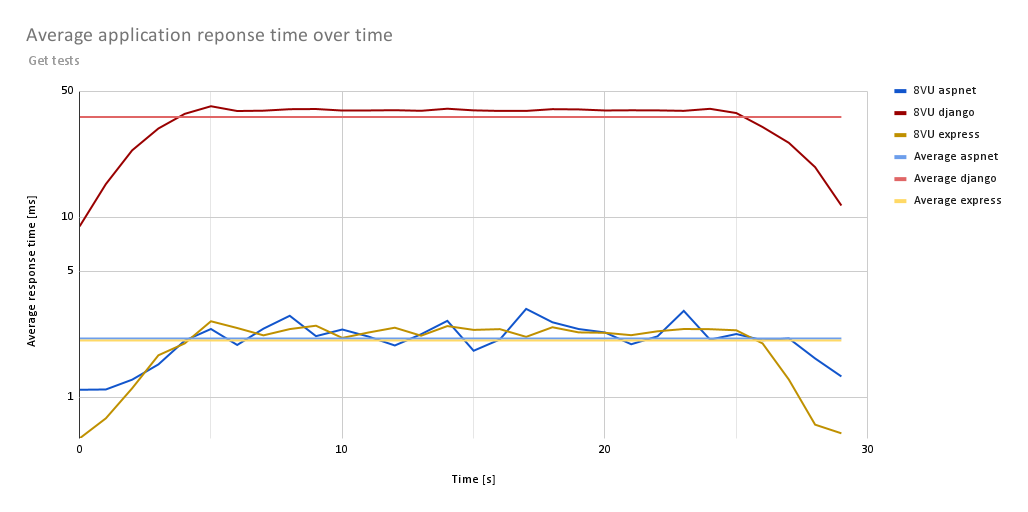
\includegraphics[width=\columnwidth]{figures/pictures/influxGraph8VU.png}
    \caption{Graph showing average response time over time in Get tests for 8 VUs}
    \label{fig:influxGraph8}
\end{figure}

\begin{figure}[H]
    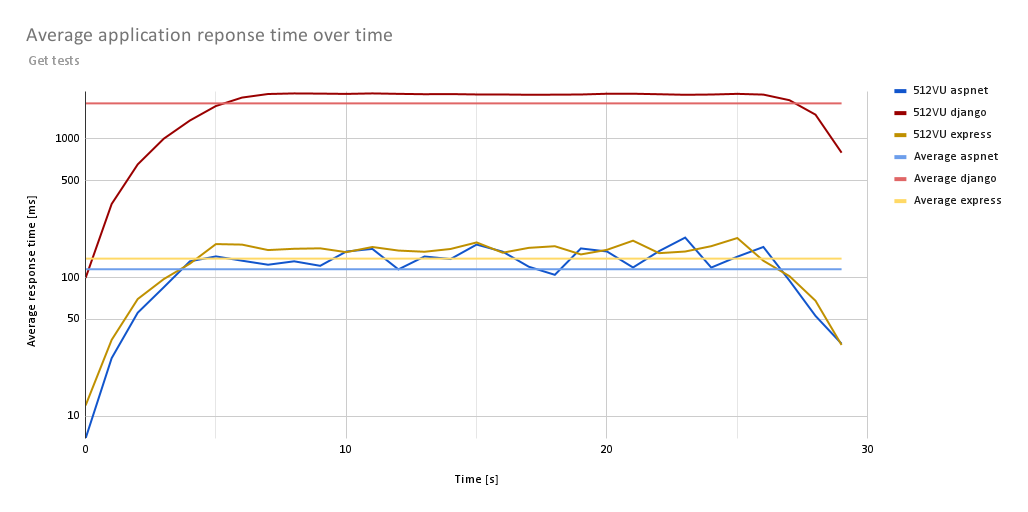
\includegraphics[width=\columnwidth]{figures/pictures/influxGraph512VU.png}
    \caption{Graph showing average response time over time in Get tests for 512 VUs}
    \label{fig:influxGraph512}
\end{figure}


From the results showing average response time over time a standard deviation was calculated between the 5th and 25th second of the test (ramp up and ramp down times were excluded). As the table \ref{tab:stdev} shows, on high load for all endpoints except updating models Express.js had the lowest standard deviation. This means that the application created on Express.js for deleting, retrieving and creating objects in the database is the most stable of the three.

\FloatBarrier
\begin{table}[!htp]\centering
    \caption{Standard deviation in milliseconds from average response times between 5th and 25th second of the tests}\label{tab:stdev}
    \scriptsize
    \begin{tabular}{lrrrrr}\toprule
        test    & concurrency & aspnet & django & express \\\midrule
        delete  & 1           & 0.03   & 0.09   & 0.05    \\
        delete  & 8           & 0.25   & 1.85   & 0.14    \\
        delete  & 32          & 1.41   & 6.55   & 1.01    \\
        delete  & 128         & 8.99   & 48.77  & 3.08    \\
        delete  & 512         & 30.23  & 273.23 & 19.99   \\
        get     & 1           & 0.03   & 0.10   & 0.02    \\
        get     & 8           & 0.35   & 0.71   & 0.15    \\
        get     & 32          & 1.29   & 2.87   & 0.84    \\
        get     & 128         & 5.83   & 26.00  & 3.17    \\
        get     & 512         & 22.20  & 178.41 & 12.63   \\
        getMany & 1           & 4.45   & 1.82   & 2.39    \\
        getMany & 8           & 6.98   & 4.58   & 4.33    \\
        getMany & 32          & 13.46  & 13.21  & 5.75    \\
        getMany & 128         & 23.14  & 62.05  & 4.51    \\
        getMany & 512         & 40.51  & 534.71 & 12.93   \\
        post    & 1           & 0.02   & 0.11   & 0.04    \\
        post    & 8           & 0.06   & 1.67   & 0.05    \\
        post    & 32          & 0.74   & 7.45   & 0.55    \\
        post    & 128         & 2.69   & 47.31  & 1.79    \\
        post    & 512         & 13.92  & 298.39 & 5.09    \\
        put     & 1           & 0.02   & 0.12   & 0.07    \\
        put     & 8           & 0.25   & 1.03   & 0.25    \\
        put     & 32          & 1.50   & 8.84   & 1.05    \\
        put     & 128         & 6.95   & 44.66  & 4.51    \\
        put     & 512         & 16.53  & 367.09 & 16.90   \\
        \bottomrule
    \end{tabular}
\end{table}
\FloatBarrier


\section{Security}
\subsection{Security Misconfiguration}
\subsubsection{Django specific variables}
Django has one configuration file, generated automatically at the project creation. At the starting lines of settings.py a few important variables and comments are placed (listing \ref{lst:djangoSettings}).
\begin{lstlisting}[language=Python,caption={Fragment of unchanged newly generated Django settings file},breaklines=true,label={lst:djangoSettings}]
    # Quick-start development settings - unsuitable for production
    # See https://docs.djangoproject.com/en/3.1/howto/deployment/checklist/
    
    # SECURITY WARNING: keep the secret key used in production secret!
    SECRET_KEY = 'k!vv90$1&z+%fhv!+c^#1pfe_f&jim&tv7$yk%d9wspv=)#$x+'
    
    # SECURITY WARNING: don't run with debug turned on in production!
    DEBUG = True
    
    ALLOWED_HOSTS = []
\end{lstlisting}


As we can see, the creators of Django clearly want the developers to prevent some security vulnerabilities, by placing \lstinline{SECURITY WARNING} comments above two crucial variables - \lstinline{SECRET_KEY} and \lstinline{DEBUG}.
As the documentation mentions, \lstinline{SECRET_KEY} is used in \cite{djangoSecretKey} \cite{djangoSigning}:
\begin{itemize}
      \item Generating session tokens
      \item Generating password reset tokens
      \item Ensuring that data passed from django forms is not changed
      \item Generating secret URLs for temporary access to a protected resource (for example a file)
      \item And any other cryptographic signing, unless a developer provides a different key 
\end{itemize}
All of them are very serious risks and should be avoided by any means. App created for this research is tiny and does not have any serious logic other than working on a database model, so cryptographic signing is not used at all. For any commercial applications leaking this variable could cause a lot of harm.
The second risky variable - \lstinline{DEBUG} - is responsible for turning on and off a debug mode. When set to True, whenever an error happens Django will display a detailed traceback, including parts of the applications source code and environment variables (such as Django settings).
Django developers thought about it being a little secure in case of accidental leakage by excluding from the message variables containing the following strings:
\begin{itemize}
      \item API,
      \item KEY,
      \item PASS,
      \item SECRET,
      \item SIGNATURE,
      \item TOKEN.
\end{itemize}
\begin{figure}[H]
    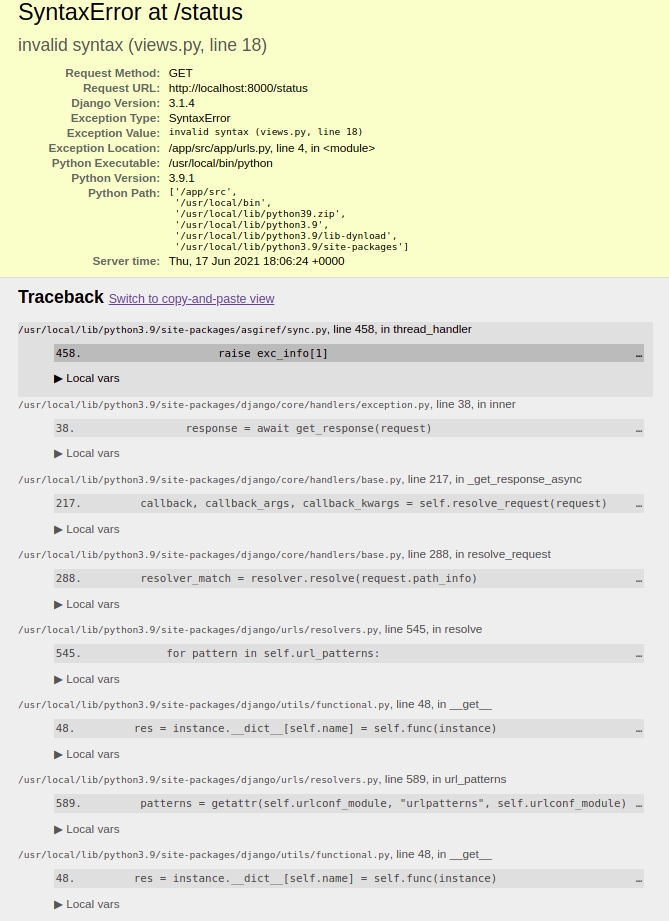
\includegraphics[width=\columnwidth]{figures/pictures/djangoStackTrace.jpg}
    \caption{Stack trace shown on error with DEBUG=True in Django}
    \label{fig:djangoStackTrace}
\end{figure}

\begin{figure}[H]
    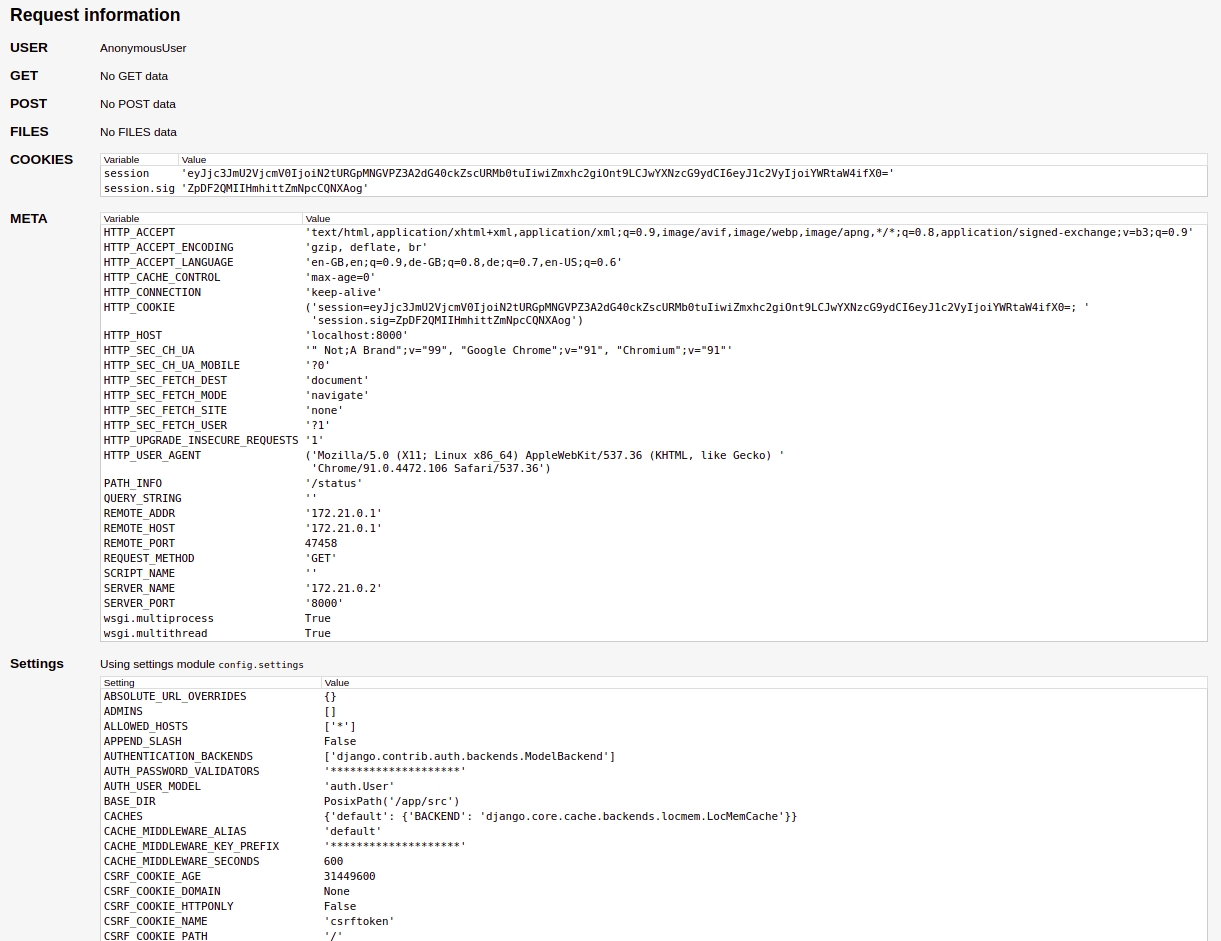
\includegraphics[width=\columnwidth]{figures/pictures/djangoRequestDetails.jpg}
    \caption{Request details and Django settings shown on error with DEBUG=True in Django}
    \label{fig:djangoRequestDetails}
\end{figure}


Third important variable that cannot be forgotten is \lstinline{ALLOWED_HOSTS} (without \lstinline{SECURITY WARNING} comment, as it is set to an empty array by default). This variable is meant to be a list of strings presenting host names that Django can send responses to. If a given host is not on the list and tries to request a resource, response with status 400 is sent immediately. When \lstinline{DEBUG} is set to True and this variable is empty, the only way to get response from the app is by requesting localhost.

To help the developers, Django offers a command \lstinline{python3 manage.py check --deploy} command. It includes a few essential steps to prepare the environment for production without security risks.
\begin{lstlisting}[keywordstyle=\color{black},caption={Warnings shown by Django check deploy command on fresh project},breaklines=true,label={lst:djangoCheckDeploy}]
    > python3 manage.py check --deploy
    System check identified some issues:
    
    WARNINGS:
    ?: (security.W004) You have not set a value for the SECURE_HSTS_SECONDS setting. If your entire site is served only over SSL, you may want to consider setting a value and enabling HTTP Strict Transport Security. Be sure to read the documentation first; enabling HSTS carelessly can cause serious, irreversible problems.
    ?: (security.W008) Your SECURE_SSL_REDIRECT setting is not set to True. Unless your site should be available over both SSL and non-SSL connections, you may want to either set this setting True or configure a load balancer or reverse-proxy server to redirect all connections to HTTPS.
    ?: (security.W012) SESSION_COOKIE_SECURE is not set to True. Using a secure-only session cookie makes it more difficult for network traffic sniffers to hijack user sessions.
    ?: (security.W016) You have 'django.middleware.csrf.CsrfViewMiddleware' in your MIDDLEWARE, but you have not set CSRF_COOKIE_SECURE to True. Using a secure-only CSRF cookie makes it more difficult for network traffic sniffers to steal the CSRF token.
    ?: (security.W018) You should not have DEBUG set to True in deployment.
    ?: (security.W020) ALLOWED_HOSTS must not be empty in deployment.
    
    System check identified 6 issues (0 silenced).
\end{lstlisting}


\subsubsection{Common problems}
There are a few things to remember when releasing any application to the world.
\begin{enumerate}
      \item Always use newest versions of frameworks and packages.

            Every external dependency that is brought to the project may be adding an additional vulnerability to the application. That is what vulnerability databases were created for - when someone discovers a problem in a given software it is often added to a list including vulnerability description and version of the faulty package. Snyk can be an example of a vulnerability \acrshort{db}. \cite{snyk}

      \item Do not configure the application to run as root

            This opens a window for the attacker to run malicious scripts or starting new child processes on a server.

      \item Limit request body size

            With unlimited sizes in body the server can be repetitively requested with large input payload, which could cause a server crash through running out of memory or keeping the processor busy. \cite{securityMisconfiguration}
\end{enumerate}

\subsection{Injection}
Prepared applications were tested with user creation requests containing malicious \acrshort{sql} statements. Request body was prepared based on logs shown in \ref{lst:sqlPost}, to check if the input string could be terminated and any other \acrshort{sql} statement could be executed.
\begin{figure}[H]
    \centering
    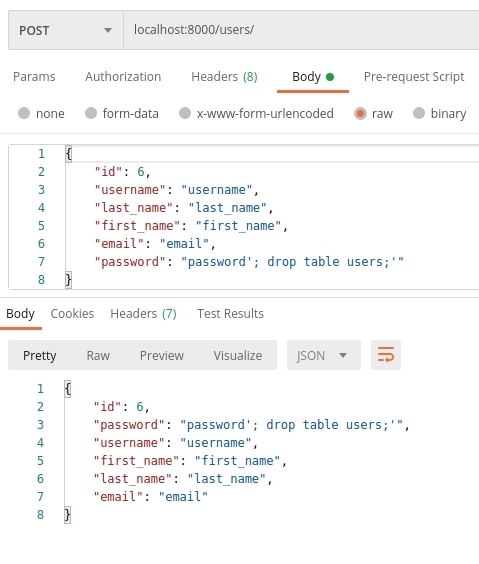
\includegraphics[width=0.6\columnwidth]{figures/pictures/injectionRequest.jpg}
    \caption{Injection request used in security tests and response from Express.js}
    \label{fig:injectionRequest}
\end{figure}


\acrshort{sql} logs of the requests are placed in listings \ref{lst:aspnetInjectionLog}, \ref{lst:expressInjectionLog} and \ref{lst:djangoInjectionLog}. As shown, the characters that could cause the harm in this case are escaped (single quotes are doubled) in all applications, resulting in creating the user normally with password containing the malicious code.
\begin{lstlisting}[caption={Log of ASP.NET injection request},breaklines=true,label={lst:aspnetInjectionLog}]
    LOG:  statement: INSERT INTO users (id, email, first_name, last_name, password, username) VALUES ($1, $2, $3, $4, $5, $6) RETURNING id
    DETAIL: parameters: $1 = 5, $2 = 'email', $3 = 'first_name', $4 = 'last_name', $5 = 'password''; drop table users;''', $6 = 'username'
\end{lstlisting}

\begin{lstlisting}[caption={Log of Express injection request},breaklines=true,label={lst:expressInjectionLog}]
    LOG:  statement: INSERT INTO users ("id", "password", "username", "first_name", "last_name", "email") VALUES(5, 'password''; drop table users;''', 'username', 'first_name', 'last_name', 'email') RETURNING *
\end{lstlisting}

\begin{lstlisting}[caption={Log of Django injection request},breaklines=true,label={lst:djangoInjectionLog}]
    LOG:  statement: INSERT INTO "app_myuser" ("id", "password", "username", "first_name", "last_name", "email") VALUES (5, 'password''; drop table "app_myuser";''', 'username', 'first_name', 'last_name', 'email') RETURNING "app_myuser"."id"
\end{lstlisting}


Additional two security test were performed, this time using path and query parameters. Retrieving users from the database required to put a user id in path, and retrieving multiple users required limit and offset variables - string termination sign was added to the values of the inputs to see the applications reaction.
\begin{figure}[H]
    \centering
    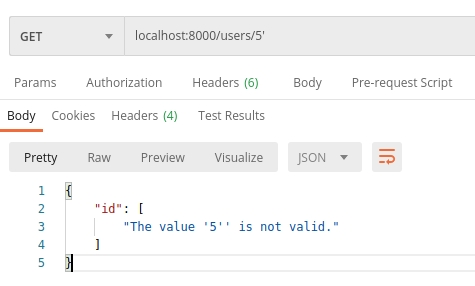
\includegraphics[width=0.7\columnwidth]{figures/pictures/getInjectionRequest.jpg}
    \caption{Get injection request used in security tests and response from ASP.NET}
    \label{fig:getInjectionRequest}
\end{figure}

\begin{figure}[H]
    \centering
    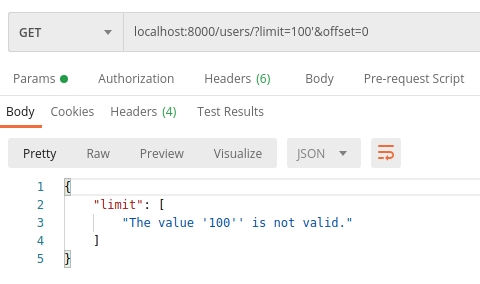
\includegraphics[width=0.7\columnwidth]{figures/pictures/getManyInjectionRequest.jpg}
    \caption{GetMany injection request used in security tests and response from ASP.NET}
    \label{fig:getManyInjectionRequest}
\end{figure}


\begin{itemize}
      \item ASP.NET Core in both cases responded with invalid request response
            \begin{itemize}
                  \item Get: \lstinline{"id": ["The value '5'' is not valid."]}
                  \item GetMany: \lstinline{"limit": ["The value '100'' is not valid."]}
            \end{itemize}
      \item Express tried to convert both variables into integers, which in this case was not successful (input became \acrshort{nan}), and application stopped executing the function and returned invalid request response.
      \item Django get function reacted similarly to ASP.NET, it returned invalid request response \lstinline{"detail": "Not found."}. With limit offset query it did not parse the limit argument properly and replaced it with default value instead.
\end{itemize}

Further research shown that the \acrshort{sql} injection can happen in these frameworks with careless developers. All applications provide functions which allow to perform raw \acrshort{sql} queries on the database. If a developer uses this function in the code and forgets to escape variables that include the user input results in an application that could be easily exploited.

\subsection{Insufficient logging}

Lack of logging in the code may result in not knowing about the breach in the system and suspicious behavior may go unnoticed. This section is going to describe most popular logging solutions for given applications.

\subsubsection{Django}

Django has one main logging tool, which is built in Python logging system. It consists of a few parts:
\begin{itemize}
      \item loggers, which are instances that can register messages for processing,
      \item handlers, which describe what happens with each message in a logger,
      \item filters, which gives control about filtering messages to bass from logger to handler,
      \item and formatters, which state how a log message should be written to output.
\end{itemize}
All these settings are to be configured within Django main config file \lstinline{settings.py} and after preparing the few lines of configuration they are ready to use.

Another option to use is Django-Automated-Logging package, which automatically tracks changes in our project, like model modifications or user requests.

To help with keeping track of the logs Django-Log-Viewer package may be added, which allows to browse and filter all logged messages in a built in Django admin panel.

\subsubsection{ASP.NET}

C\# offers a package named Microsoft.Extensions.Logging, which instance of logger can be attached directly to ASP.NET Core controllers and used in functions inside. What is more, it also can be added as middleware in the Program.cs file. They can be configured in many ways - in configuration file appsettings.json developers can specify different kinds of loggers that they intend to use in their application, specify their log level (to filter logs at later stages of development) or even specify log levels for modules that the application is using.

\subsubsection{Express.js}

Express.js \acrshort{npm} module named debug for logging information about routes, middlewares, requests and responses. Logs are disabled by default and to be turned on the application should be started with environment variable \lstinline{DEBUG=express:*}.

To have more detailed logging external packages can be added. Winston is the most popular one, with almost 6 million weekly downloads at the moment of writing. A logger can be defined manually with custom configuration (or default can be used) and added as middleware or used directly in the function we want to log.

\section{Lines of code}

Process of developing the applications was different for each framework, that is why it was decided to compare the written applications with tool named \acrshort{cloc}, that counts the lines of code in given directories. After excluding the configuration files and auto-generated migration files, the results are as follows:
\begin{enumerate}
      \item Django - 75 lines of code,
      \item Express.js - 156 lines of code,
      \item ASP.NET - 182 lines of code.
\end{enumerate}
